\section{Carbon Fiber Filament}

\indent

In order to print the CFRP material, carbon fiber and a resin were combined into a CFRP filament. As in conventional FDM printing, the CFRP filament is extruded by driving it through a heated nozzle. ABS plastic was chosen as the matrix material for this filament for several reasons. First, ABS has already successfully been combined with chopped carbon fiber in FDM filaments. Second, ABS does not require post-processing to reach full strength, as epoxy-based pre-impregnated carbon fiber composites do. In all filament development methods a 1K carbon fiber tow (shown in Figure~\ref{fig:carbon-fiber-spool}) was utilized.\\

\begin{figure}[htp]
    \centering
    \includegraphics[width=0.5\textwidth]{./figures/carbon-fiber-spool}
    \caption{The 1K carbon fiber spool.}
    \label{fig:carbon-fiber-spool}
\end{figure}

\subsection{Production Methods}

\indent

Two proudction methods were explored for developing a CFRP filament. The first was pultrusion, an efficient fabrication method widely used to manufacture fiber-reinforced structural members. The second was a slurry dipping method, a tedious process where fibers were guided through a solution containing ABS, which would air dry onto the fibers and provide full fiber wet-out.\\

\subsubsection{Pultrusion}

\indent

A 3Doodler handheld 3D printing device was employed in pultrusion tests. The 3Doodler's feed motor was disabled, and then a bundle of carbon fiber and an ABS rod were simultaneously fed through the 3Doodler's heater and nozzle. The combined materials were manually drawn through from the exit end of the nozzle. This process is shown in Figure~\ref{fig:pultrusion-vid}. In the resulting filament, the carbon fiber bundle and the ABS adhered together well. However, due to the high viscosity of the heated ABS, most of the individual carbon fibers were not in contact with the ABS. Additionally, the fiber is not centered within the new CFRP filament, which is necessary printing.\footnote{Fibers located on the outside of the CFRP filament encounter a no-slip condition when entering the heated nozzle and subsequently never leave the nozzle with the ABS.} This effect is visible in Figure~\ref{fig:pultruded-scope}.\\

\begin{figure}[h!]
    \centering
    \includegraphics[width=0.4\textwidth]{./figures/pultrusion-vid}
    \caption{The experimental pultrusion setup, using the 3Doodler.}
    \label{fig:pultrusion-vid}
\end{figure}

\begin{figure}[h!]
    \centering
    \includegraphics[width=0.6\textwidth]{./figures/pultruded-scope}
    \caption{Pultruded filament sample, magnified 10x under a microscope.}
    \label{fig:pultruded-scope}
\end{figure}

\clearpage

\subsubsection{Slurry Dipping}

\indent

Good fiber wet-out is critical to the performance of fiber composites, so another filament production method was explored. In the new procedure, achieving complete wet-out was prioritized. ABS plastic was dissolved in acetone to make a slurry. A fiber guide was fabricated to guide the carbon fiber in and out of the slurry. Carbon fiber bundles were then drawn through the fiber guide and allowed to dry. The process setup is shown in Figure~\ref{fig:dipping-vid}. As the acetone evaporated from the slurry, a small amount of ABS was left on the carbon fibers. The resulting filament showed very good wet-out. A pultruded sample and a dipped sample are shown side-by-side in Figure~\ref{fig:two-samples}. \large{\textbf{SLURRY DIPPING CITE!}}\\

\begin{figure}[h!]
    \centering
    \includegraphics[width=0.8\textwidth]{./figures/dipping-vid}
    \caption{The basic slurry dipping process.}
    \label{fig:dipping-vid}
\end{figure}

\begin{figure}[h!]
    \centering
    \includegraphics[width=0.6\textwidth]{./figures/FilamentSample}
    \caption{A pultruded filament sample (top) and a dipped filament sample (bottom), labeled with sample numbers.}
    \label{fig:two-samples}
\end{figure}

As the more promising of the two methods, slurry dipping was explored further in attempt to create a viable CFRP filament. The dipping concept was validated with a more-or-less arbitrary amount of ABS and acetone mixed together, and with only one form of wire guide. In the making of the actual CFRP filament, multiple solution concentrations, wire guides, and other factors were experimented upon. To create the slurry solutions, various lengths of 1.75 \emph{mm} diameter ABS filament from Makerbot\footnote{\url{https://www.makerbot.com}} were chopped up and mixed with acetone. Figure~\ref{fig:slurry-making} illustrates this process. Filament was chopped up into roughly 0.5 inch lengths (Figure~\ref{fig:filament-abs-chopped}), volume markings on the containers were used to measure out acetone (Figure~\ref{fig:filament-mixture-volume-markings}), and the mixture shaken vigorously by hand until all of the ABS dissolved to create solutions of multiple concentrations. The concenterations are labeled by the length of ABS and volume of acetone use to create the mixutre. \\

%%% slurry making photos

\begin{figure}[h!]
        \centering
        \begin{subfigure}[b]{0.3\textwidth}
                \includegraphics[width=\textwidth]{./figures/filament-abs-chopped}
                \caption{Chopped ABS.}
                \label{fig:filament-abs-chopped}
        \end{subfigure}%
        \begin{subfigure}[b]{0.3\textwidth}
                \includegraphics[width=\textwidth]{./figures/filament-mixture-volume-markings}
                \caption{Volume markings.}
                \label{fig:filament-mixture-volume-markings}
        \end{subfigure}
        \begin{subfigure}[b]{0.3\textwidth}
                \includegraphics[width=\textwidth]{./figures/filament-mixtures}
                \caption{Various mixtures.}
                \label{fig:filament-mixtures}
        \end{subfigure}
        \caption{Photos of the ABS-acetone slurry-making process}\label{fig:slurry-making}
\end{figure}



%%% Dipping Method Diagrams

%\begin{figure}[h!]
%    \centering
%    \includegraphics[width=0.5\textwidth]{./figures/external-dip-diagram}
%    \caption{An illustration of a wire-guided dipping method with the guide only partially immersed in the slurry.}
%    \label{fig:external-dip-diagram}
%\end{figure}
%
%\begin{figure}[h!]
%    \centering
%    \includegraphics[width=0.5\textwidth]{./figures/internal-dip-diagram}
%    \caption{An illustration of a wire-guided dipping method with the guide fully immersed in the slurry.}
%    \label{fig:internal-dip-diagram}
%\end{figure}
%
%\begin{figure}[h!]
%    \centering
%    \includegraphics[width=0.5\textwidth]{./figures/flat-dip-diagram}
%    \caption{An illustration of the bath dipping method.}
%    \label{fig:flat-dip-diagram}
%\end{figure}

Multiple dipping methods (or guide configurations) were used while developing a viable method for creating the CFRP filament. Figure~\ref{fig:dip-diagram} shows the three setups utilized. Figure~\ref{fig:external-dip-diagram} shows a wire guide with three guide loops, one immersed in and two external to the slurry. Figure~\ref{fig:interal-dip-diagram} illustrates a guide utilized where all loops are immersed in the slurry. Figure~\ref{fig:flat-dip-diagram} pushes the definition of a guided dip and simply involves using tweezers to place the fiber into a shallow slurry bath. Of course, each method had pros and cons. For the partially immersed guide, a bit of slurry is scraped off on the exiting external loop prior to acetone evaporation, which adds less ABS per dip than the fully immersed guide. However, the fully immersed guide does not prevent the CFRP from scraping up against the walls of the container. With a steady hand an patience, this can be avoided and about the twice the mass of ABS can be added to the carbon fiber tow in the same number of passes through the slurry.The bath avoids the problem of scraping off on any surface altogether and drastically increases the speed at which a length of tow can be coated with ABS. However, a large area is exposed to ambient temperature and pressure. Without a confined box or cold outside temperature, the acetone evaporates rapidly at the surface, leaving a thin film of ABS at the surface which generates a more rectangular shaped filament after multiple passes instead of a circular cross section. \\

\begin{figure}[h!]
        \centering
        \begin{subfigure}[b]{0.3\textwidth}
                \includegraphics[width=\textwidth]{./figures/external-dip-diagram}
                \caption{Partially immersed guide.}
                \label{fig:external-dip-diagram}
        \end{subfigure}%
        ~ %add desired spacing between images, e. g. ~, \quad, \qquad, \hfill etc.
          %(or a blank line to force the subfigure onto a new line)
        \begin{subfigure}[b]{0.3\textwidth}
                \includegraphics[width=\textwidth]{./figures/internal-dip-diagram}
                \caption{Fully immersed guide.}
                \label{fig:internal-dip-diagram}
        \end{subfigure}
        ~ %add desired spacing between images, e. g. ~, \quad, \qquad, \hfill etc.
          %(or a blank line to force the subfigure onto a new line)
        \begin{subfigure}[b]{0.3\textwidth}
                \includegraphics[width=\textwidth]{./figures/flat-dip-diagram}
                \caption{Bath dipping.}
                \label{fig:flat-dip-diagram}
        \end{subfigure}
        \caption{Slurry Dippng Methods.}\label{fig:dip-diagram}
\end{figure}

%%% Filament Photos

Figure~\ref{fig:20-og} through Figure~\ref{fig:20-ng} show microscope images of CFRPs created different solutions and dipping methods. All wire-guided dipping methods created CFRP filaments with circular cross sections and a centered carbon fiber tow, both of which are required for FDM. Note that all cross sections but the bath dip show voids in the CFRP. This suggests that voids in the CFRP are frequently occurs from evaporating acetone getting trapped beneath solifying layers of ABS.  Unlike the guided methods, the bath configuration did not give a smooth surface due to the thin film phenomenon. Some defects are visible at the microscope level. From a macroscopic  level these defects are not of concern. Once in the heated portion of the extruder, these defects are melted down and disappear. Additionally, many of the defects are small in length. Large defects could affect the gripping ability of the notched screw used in the extruder mechanism but defects mainly apparent on a microscopics scale are not worrisome.\\

% external guide

\begin{figure}[h!]
        \centering
        \begin{subfigure}[b]{0.3\textwidth}
                \includegraphics[width=\textwidth]{./figures/20-og-normal}
                \caption{Length normal.}
                \label{fig:20-og-normal}
        \end{subfigure}%
        ~ %add desired spacing between images, e. g. ~, \quad, \qquad, \hfill etc.
          %(or a blank line to force the subfigure onto a new line)
        \begin{subfigure}[b]{0.3\textwidth}
                \includegraphics[width=\textwidth]{./figures/20-og-defect}
                \caption{Length defect.}
                \label{fig:20-og-defect}
        \end{subfigure}
        ~ %add desired spacing between images, e. g. ~, \quad, \qquad, \hfill etc.
          %(or a blank line to force the subfigure onto a new line)
        \begin{subfigure}[b]{0.3\textwidth}
                \includegraphics[width=\textwidth]{./figures/20-og-end}
                \caption{Cross section.}
                \label{fig:20-og-end}
        \end{subfigure}
        \caption{Microscopic views (10X) of a CFRP filament created with 20 dips using the partially immersed guide.}\label{fig:20-og}
\end{figure}

% inernal guide

\begin{figure}[h!]
        \centering
        \begin{subfigure}[b]{0.3\textwidth}
                \includegraphics[width=\textwidth]{./figures/20-ng-normal}
                \caption{Length normal.}
                \label{fig:20-og-normal}
        \end{subfigure}%
        ~ %add desired spacing between images, e. g. ~, \quad, \qquad, \hfill etc.
          %(or a blank line to force the subfigure onto a new line)
        \begin{subfigure}[b]{0.3\textwidth}
                \includegraphics[width=\textwidth]{./figures/20-ng-defect}
                \caption{Length defect.}
                \label{fig:20-og-defect}
        \end{subfigure}
        ~ %add desired spacing between images, e. g. ~, \quad, \qquad, \hfill etc.
          %(or a blank line to force the subfigure onto a new line)
        \begin{subfigure}[b]{0.3\textwidth}
                \includegraphics[width=\textwidth]{./figures/20-ng-end}
                \caption{Cross section.}
                \label{fig:20-og-end}
        \end{subfigure}
        \caption{Microscopic views (10X) of a CFRP filament created with 20 dips using the fully immersed guide.}\label{fig:20-ng}
\end{figure}

% 108 40 dip

\begin{figure}[h!]
        \centering
        \begin{subfigure}[b]{0.3\textwidth}
                \includegraphics[width=\textwidth]{./figures/filament-108-40-dip-side}
                \caption{Length.}
                \label{fig:filament-108-40-dip-side}
        \end{subfigure}
        \begin{subfigure}[b]{0.3\textwidth}
                \includegraphics[width=\textwidth]{./figures/filament-108-40-dip-end}
                \caption{Cross section.}
                \label{fig:filament-108-40-dip-end}
        \end{subfigure}
        \caption{Microscopic views (10X) of a CFRP filament created with 10 dips using the fully immersed guide in a 16\% ABS solution.}\label{fig:filament-108-40-dip-microscope}
\end{figure}

% 108 40 bath

\begin{figure}[h!]
        \centering
        \begin{subfigure}[b]{0.3\textwidth}
                \includegraphics[width=\textwidth]{./figures/filament-108-40-flat-side}
                \caption{Length.}
                \label{fig:filament-108-40-flat-side}
        \end{subfigure}
        \begin{subfigure}[b]{0.3\textwidth}
                \includegraphics[width=\textwidth]{./figures/filament-108-40-flat-end}
                \caption{Cross section.}
                \label{fig:filament-108-40-flat-end}
        \end{subfigure}
        \caption{Microscopic views (10x) of a CFRP filament created with 5 bathing rotations in a 16\% ABS solution.}\label{fig:filament-108-40-bath-microscope}
\end{figure}


%%% Dipping Results Summary

Table~\ref{tab:dipping-results} summarizes quantitative lessons learned from testing dipping configurations. 108 \emph{in} of ABS and 40 {mL} of acetone seems to be the most efficeint solution. Testing indicated indicated that this solution is close to fully saturated. After multiple dipping sessions, enough acetone had naturally evaporated when the lid was openned that a thin ABS film began to form on top of the solution and colloidal ABS chunks also formed inside the general mixture. Curiously, this solution output a similar density to a lower concentration mixture even though it required fewer dips and resulted in a larger diameter. Therefore, it can be assumed that a lower concentration solution, will result in fewer voids containing air or acetone.\\

\begin{table}[h!]
    \centering
    \begin{tabular}{p{1.5in}|p{1in}|p{0.75in}|p{0.75in}|p{0.75in}|p{0.75in}}
        Filament Formulation & Concentration of ABS, $m^3/m^3$ & Density, $kg/m^3$ & Percent Carbon Fiber, $kg/kg$ & Filament Diameter, $mm$ & ABS Added per Dip per Length, $kg/m$  \\ \hline \hline
        60 \textit{in} ABS, 40 \textit{mL} Acetone, Guided & 0.09 & 818 & 19 & 0.73 & 0.017 \\ \hline
        108 \textit{in} ABS, 40 \textit{mL} Acetone, Guided & 0.16 & 758 & 4 & 1.63 & 0.157 \\ \hline
        108 \textit{in} ABS, 40 \textit{mL} Acetone, Bath & 0.16 & 645 & 5 & 1.67 & 0.282 \\
 
    \end{tabular}
    \caption{A summary of dipping results from different slurry concentrations and guide methods.}
    \label{tab:dipping-results}
\end{table}

%%% Dipping Results Discussion

Figure~\ref{fig:filament-dipping-dried} shows a drying 108-40 filament dipped ten times. At a low number of dips the CFRP filament is very brittle (ie, rather than smoothly bending it will contain harsh corners). However, as more ABS is added to the filament, it becomes significantly more ductile and nicely bends, as shown in Figure~\ref{fig:filament-dipping-dried}. Figure~\ref{fig:filament-dipping-shear} shows one of the most common issues that arose with wire-guided dipping. As more and more ABS was added to the carbon fiber tow, it became more susceptible to shearing off. Simply brushing up agains the edge of the container prior to being let to dry (about three hours was required for setting a 1 foot segment) could tear off chuncks of plastic, rendering the CFRP useless. A steady hand with the fully immersed wire guide was the only way to avoid this issue.\\

\begin{figure}[htp]
    \centering
    \includegraphics[width=0.8\textwidth]{./figures/filament-dipping-dried}
    \caption{A drying CFRP filament.}
    \label{fig:filament-dipping-dried}
\end{figure}

\begin{figure}[htp]
    \centering
    \includegraphics[width=0.8\textwidth]{./figures/filament-dipping-shear}
    \caption{CFRP filament with ABS sheared off from external guides.}
    \label{fig:filament-dipping-shear}
\end{figure}

\clearpage

\subsection{Mechanical Testing}

\indent

Tensile tests were performed on the filament samples that were produced using the pultrusion and dipping methods. The test gathered data useful for assessing the strength and stiffness of potential filaments and also provided a collection of material data pertinent to the finite element analysis.\\

\subsubsection{Setup}

\indent

An Instron mechanical testing machine (Figure~\ref{fig:intstron-overview}) was used for these tensile tests. Short lengths of filament (roughly 2 in) were cut from larger samples for testing. Due to the small, slippery,  and flexible nature of the filament samples, the regular serrated jaw inserts of the Instron tensile test jaws could not be used alone to secure the samples. Instead of clamping the samples directly in the jaws, the samples were securely mounted to aperture cards using melted ABS. The ends of the card were folded over the filament. Once clamped in the serrated jaws, the cardboard protected the filament from the jaws and held it securely in place. The card also assisted in aligning the filament with the jaws. Once clamped, the exposed portion of the card was cut with scissors, and the test was started. Figure~\ref{fig:instron-setup} shows the setup of the aperture cards in the Intson jaws. For concistency all samples were loaded until failure (carbon fiber fracture) at an elongation rate of 2 \textit{mm/min} the force applied output as the dependent variable in the system. Figure~\ref{fig:filament-card-after-instron} shows a fractured filament and the apeture card ABS glue setup.\\

\begin{figure}[h!]
    \centering
    \includegraphics[width=0.5\textwidth]{./figures/intstron-overview}
    \caption{A photo of the Instron machine.}
    \label{fig:intstron-overview}
\end{figure}

\begin{figure}[h!]
        \centering
        \begin{subfigure}[b]{0.3\textwidth}
                \includegraphics[width=\textwidth]{./figures/filament-instron-1}
                \caption{Installed in jaws.}
                \label{fig:filament-instron-1}
        \end{subfigure}
        \begin{subfigure}[b]{0.3\textwidth}
                \includegraphics[width=\textwidth]{./figures/filament-instron-2}
                \caption{Cut card ready for testing.}
                \label{fig:filament-instron-2}
        \end{subfigure}
        \caption{A filament specimen loaded in the Instron for a tensile test.}\label{fig:instron-setup}
\end{figure}

\begin{figure}[h!]
    \centering
    \includegraphics[width=0.5\textwidth]{./figures/filament-card-after-instron}
    \caption{A photo of a filament specimen after tensile testing.}
    \label{fig:filament-card-after-instron}
\end{figure}

\clearpage

\subsubsection{Results}

\indent

The tensile tests performed on the filament samples provide insight into some of their basic mechanical properties. A representative tensile test extension-load plot is provided in Figure~\ref{fig:instron-sample}. The CFRP samples showed fairly linear behavior before failing. Table~\ref{tab:test-results} compares the estimated ultimate tensile strength, stiffness, and density of two\footnote{Nearly a dozen samples were created. These two filaments selected for the table exhibited the most reasonable properties.} filament samples with those of ABS, carbon fiber, and aluminum 6061. The properties of aluminum were included for comparison because CFRP materials are often used to replace aluminum parts. Unfortunately, the result shown do not included the rigorously develped dipped CFRP filament. Increased amounts of ABS led to the carbon fiber tow simply shearing off of the ABS in every tensile test so no realistic tensile data could be gathered. However, the results are promising: both the pultruded and dipped filament samples are lighter and have ultimate tensile strength's on the order of that of aluminum 6061, although they are not as stiff.\\

\begin{figure}[htp]
    \centering
    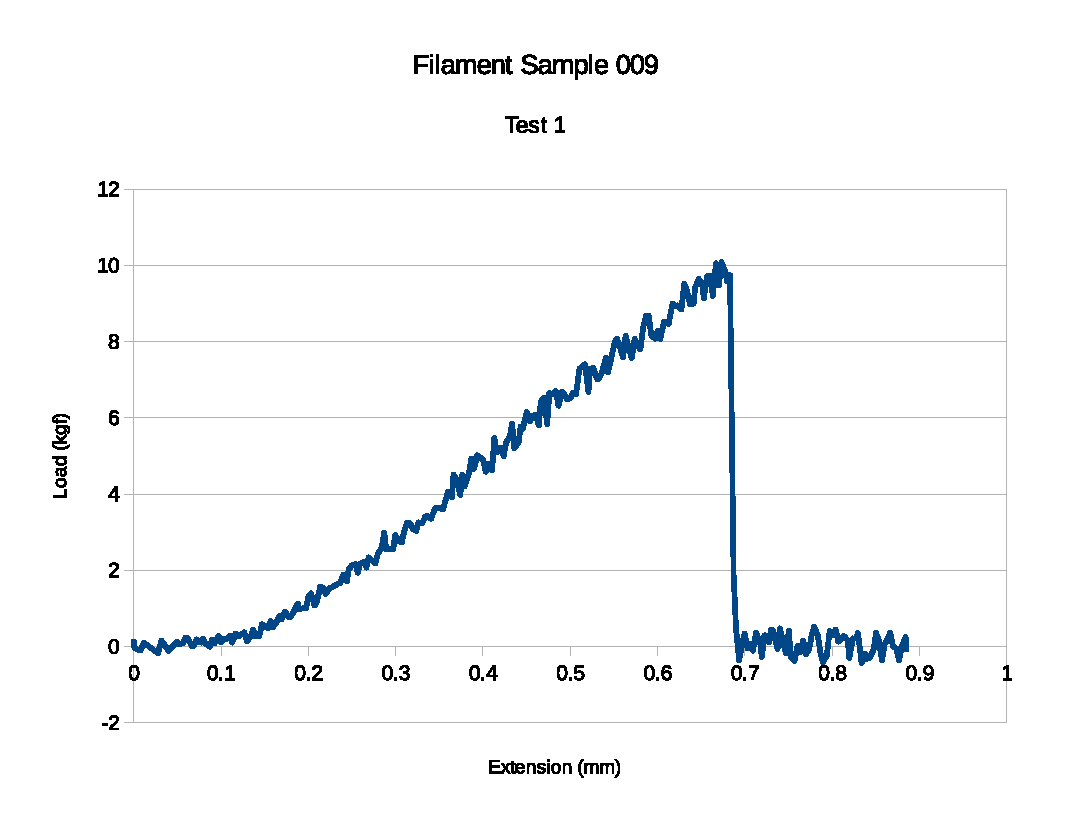
\includegraphics[width=0.8\textwidth]{./figures/009T1-instron-data}
    \caption{Sample tensile test data for a slurry-dipped filament sample.}
    \label{fig:instron-sample}
\end{figure}

\begin{table}[h]
    \centering
    \begin{tabular}{lcccc}
        Material           & Ultimate Tensile Strength (MPa)   & Stiffness (GPa)    & Density ($ kg/m^{3} $)  \\ \hline
        ABS                & 53                                & 2.3                & 1040 \\
        Carbon Fiber       & 3750                              & 231                & 1750 \\
        Aluminum 6061      & 310                               & 68.9               & 2700 \\
        Pultruded Filament & 313                               & 13.4               & 1354 \\ 
        Dipped Filament\tablefootnote {This is a representative dipped filament from initial test, not from thorough investigations of different diping methods.} & 690                               & 19.6 & 1567 \\
    \end{tabular}
    \caption{Preliminary CFRP filament test results, as compared to its constituents and to aluminum.}
    \label{tab:test-results}
\end{table}

\clearpage

\subsection{Print Testing}

\indent

All of the method testing resulted in a 10 times dipped (using a fully immersed guide) tow in 16\% ABS solution being the most viable CFRP filament. This filament contained relatively quick ABS coating times, a reasonable diameter equivalent to that of the purchased Makerbot filament, and a centered carbon fiber tow. Prior to printing with the FANUC mounted extruder, the short length of CFRP filament was test printed using the 3Doodler. Figure~\ref{fig:filament-print-test} shows before and after photos of the test. To successfully print with the CFRP filament, ABS must be striped off the very front of the strand, the carbon fiber inserted through a room temperature nozzle and glued to the print surface with the ABS slurry to create tension. Once printing, the hardened, extruded filament maintains the forward tension. This tension is necessary for printing to ensure that the filament aligns with the nozzle outlet hole and does not buckle under the pressure of heated ABS in the nozzle. The after shot (Figure~\ref{fig:filament-print-3doodler-after}) shows two prints (black) and the filament removed from the extruder nozzle (orange). Figure~\ref{fig:filament-print-3doodler-during} shows an image of the printing in action and Figure~\ref{fig:filament-extrude} shows a close up photo of one of the printed strands. Unlike the CFRP filament which appeared to contain a substain amount of ABS, the printed strand appear to be mostly carbon fiber. This is not necessarily a bad thing, but only physically printing large parts will determine whether or not this is a sufficient amount of matrix material. \\

\indent

\begin{figure}[h!]
        \centering
        \begin{subfigure}[b]{0.3\textwidth}
                \includegraphics[width=\textwidth]{./figures/filament-print-3doodler-before}
                \caption{Before.}
                \label{fig:filament-print-3doodler-before}
        \end{subfigure}
        \begin{subfigure}[b]{0.3\textwidth}
                \includegraphics[width=\textwidth]{./figures/filament-print-3doodler-after}
                \caption{After.}
                \label{fig:filament-print-3doodler-after}
        \end{subfigure}
        \caption{Before and after shots of print testing with the CFRP filament.}\label{fig:filament-print-test}
\end{figure}

\begin{figure}[htp]
    \centering
    \includegraphics[width=0.5\textwidth]{./figures/filament-print-3doodler-during}
    \caption{Test printing the CFRP filament with a 3Doodler.}
    \label{fig:filament-print-3doodler-during}
\end{figure}

\begin{figure}[htp]
    \centering
    \includegraphics[width=0.8\textwidth]{./figures/filament-extrude}
    \caption{A close up photo of the filament printed with the 3Doodler}
    \label{fig:filament-extrude}
\end{figure}

A tensile test of the printed CFRP filament was perform to compare its properties to the non-printed filament. Table~\ref{tab:printed-filament-results} presents this data and shows that all values are on the same order as they were prior to printing. This results validates the use of inital tensile test data as material properties for finite element analysis since there is little change.\\

\begin{table}[h]
    \centering
    \begin{tabular}{lcccc}
        Material           & Ultimate Tensile Strength (MPa)   & Stiffness (GPa)    & Failure Strain (\%)  \\ \hline
		Printed Filament & 338 & 7.63 & 4.44
    \end{tabular}
    \caption{Tensile test results for the printed CFRP filament}
    \label{tab:printed-filament-results}
\end{table}

\clearpage

\subsection{Future Suggestions}

\indent

Although a viable CFRP filament was created, the process by which it was manufactured contains much room for improvement. Primarily, the current dipping process is tediously slow. It takes nearly one hour to coat approximately two feet of tow and additonally drying time. While Cooper does not currently contain coating resources, it would be best to acquire equipment that can produce this CFRP en mass or locate a service that can efficiently coat the fibers for a reasonable cost. Previous research into CFRP development even mentions the use of advanced venturi machines in plastic baths to ensure complete fiber wet-out and tow centering \large{\textbf{CITE NASA}. Going forward large lengths of this CFRP will be required for small parts and even longer lengths required for large prints; coating by hand will not be a fast enough option.